\documentclass{article}
\usepackage{amsmath, amsthm, amssymb, amsfonts, bm}
\usepackage{graphicx}
\usepackage[T1]{fontenc}
\usepackage[utf8]{inputenc}
\usepackage[a4paper]{geometry}
\usepackage{fancyhdr}
\usepackage[algo2e]{algorithm2e}
\fontfamily{cmr}

\title{DD2424 - Assignment 2}
\author{Oskar Stigland \\ stigland@kth.se}

\pagestyle{fancy}
\fancyhf{}
\rhead{stigland@kth.se}
\lhead{DD2424 - Deep Learning in Data Science}
\rfoot{Page \thepage}

\begin{document}
%\maketitle

	\begin{titlepage}
		\begin{center} 
			
			\rule{\linewidth}{0.5mm}\\[0.5 cm]
			{ \huge \bfseries DD2424 - Assignment 2}\\[0.3 cm] % Title of your document
			\rule{\linewidth}{0.5mm}\\[1 cm]
					
			\small\vfill
			\begin{center}
			\centering
			{\large \bfseries \textsc{Summary}}\\
			\vspace{1cm}
			\begin{minipage}{10cm}
				
				I have implemented the cyclical learning rate with a coarse $\lambda$ search, followed by a finer $\lambda$ search, for which I achieved a final testing accuracy of $51.80$\% when training the network for $5$ cycles with all of the training observations (except a small subset for validation) and \texttt{ns} $=500$. For the finer $\lambda$ search, I used $\lambda_{\text{min}} = -5$ and $\lambda_{\text{max}} = -3$ when sampling the exponent for calculating $\lambda$. Additionally, I have also completed the bonus problems.\\\\
%
	The code for the assignment has been written in \texttt{python}. I have implemented the neural network as a class. For the hand-in, all of the code has been put toghether in a main file with all the functions and the class declared at the top. For the hand-in, I have also commented out the saving of generated figures and results in JSON files, as well as omitting some of the case-specific testing and gradient testing.
			\end{minipage}
			\end{center}
			\large\vfill
						

		\end{center}	
		
		\begin{minipage}{0.4\textwidth}
			\begin{flushleft} \large
				%\emph{Student:}\\
				Oskar \textsc{Stigland}\\
				DD2424\\
				Spring 2023
			\end{flushleft}
		\end{minipage}	

	\end{titlepage}

\newpage

\subsection*{Checking gradients}

	In order to validate the anaytic gradient computations, I compared the analytically computed gradients with numerically computed gradients
	\begin{itemize}
		\item[(a)] a subset of the weights of a large subset of the training data, and
		\item[(b)] all of the weights on a small subset of the training data
	\end{itemize}
	using $h = 10^{-5}$.  For both (a) and (b), I got that
	$$\vert\vert \nabla_{\bm{w}} \bm{J} - \nabla_{\bm{w}} \bm{J}^{\text{numerical}} \vert\vert < 10^{-10}, \quad \forall\bm{w} \in \bm{W}$$
	where $\bm{W}$ is the full set of weights, including also the weights in the bias vector. Then, I also attempted to train the network on a small subset of the training data with $\vert D\vert = 100$ and $500$ epochs, not using any regularization. For this procedure, I got the following results:
	\begin{figure}[h!]
		\centering
		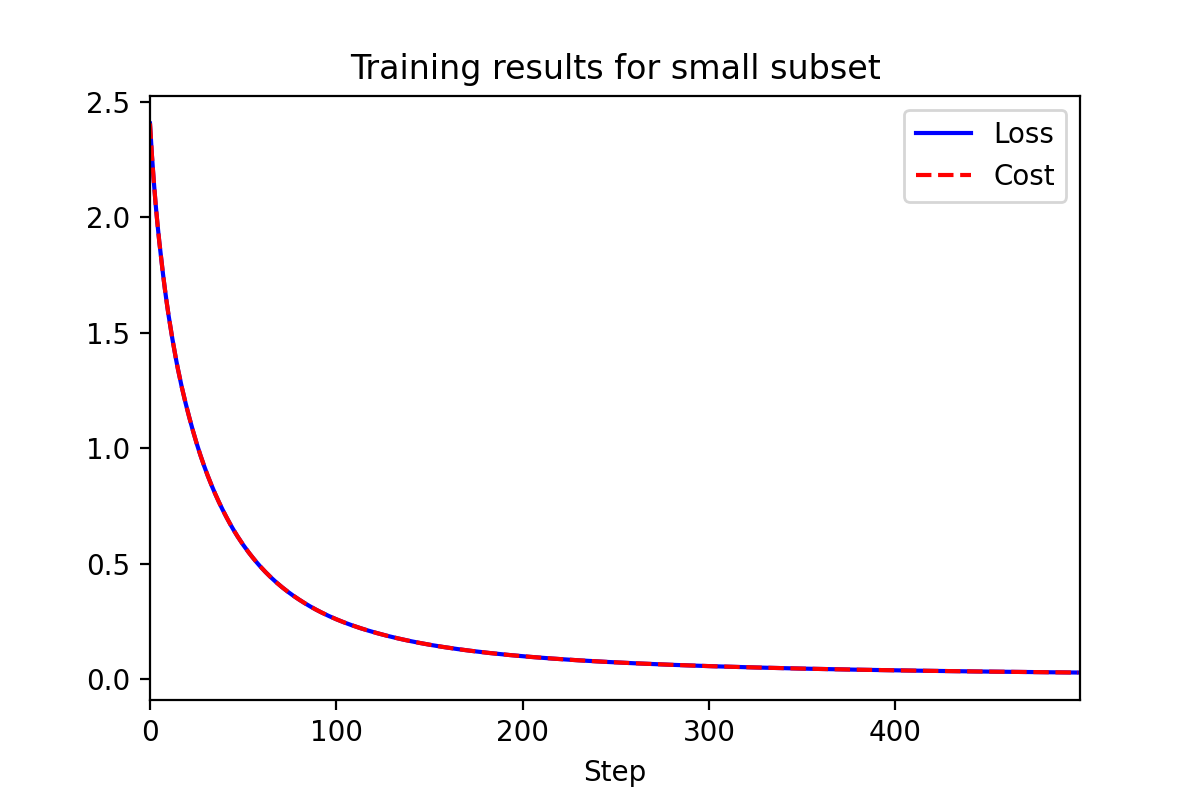
\includegraphics[width=6cm]{../plots/grad_test.png}
		\caption{Loss and cost for $\eta=0.01$, $\lambda=0.0$, on $D\subset \bm{X}$, $\vert D\vert = 100$}
	\end{figure}\\
	Thus, I am confident the analytically computed gradients are indeed correct. They are identical to the numerically computed gradients up to an acceptable accuracy and the model clearly converges to a solution when trained on a small subset of the data, indicating that the gradient calculations are stable.

\subsection*{Training with cyclical learning rates}
	For the initial parameter settings, i.e. using \texttt{nt}$=500$ for $1$ cycle and then \texttt{nt}$=800$, and $3$ cycles, the network achieves an accuracy on the testing data of $47.09$\% and $48.34$\%, respectively. The results ara shown in Figure $2$ and $3$. Overall, there are clear cyclical components in all metrics and the results seem to agree with those shown in Figure $3$ and $4$ of the assignment description.
	\begin{figure}[h!]
		\centering
		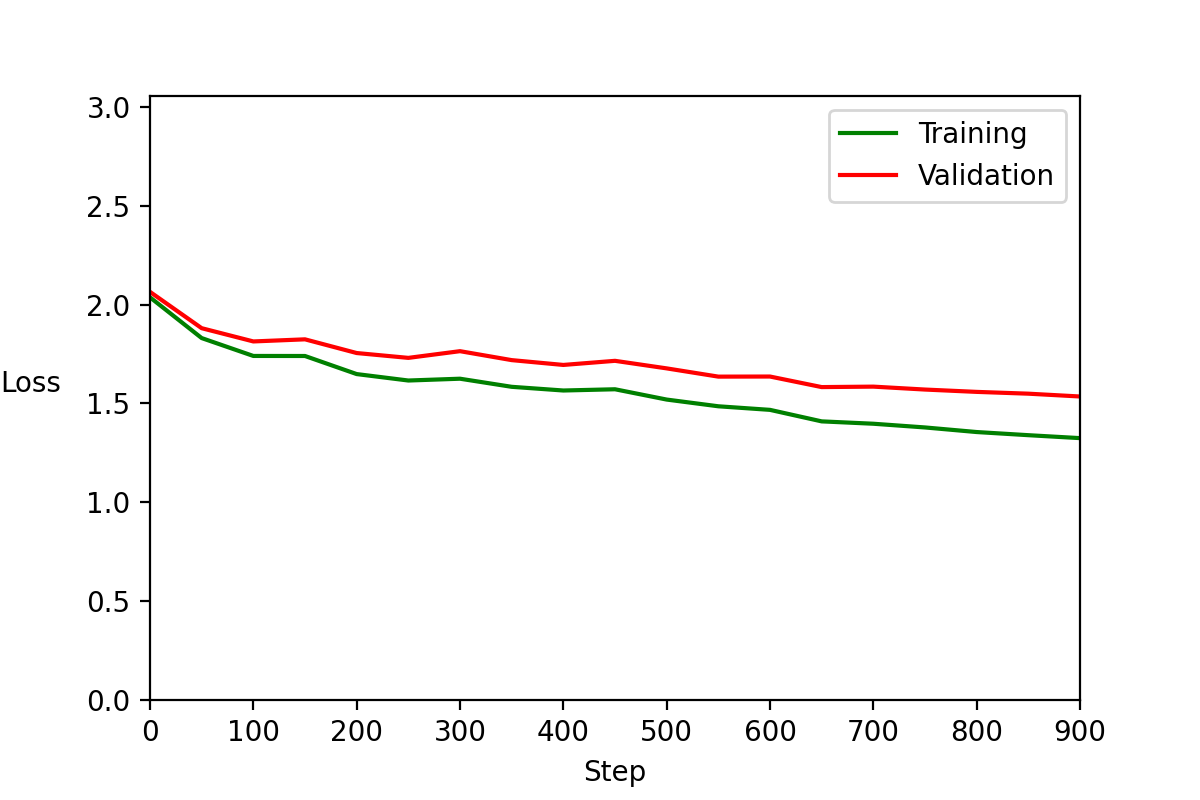
\includegraphics[width=4cm]{../plots/loss_init_v1.png}
		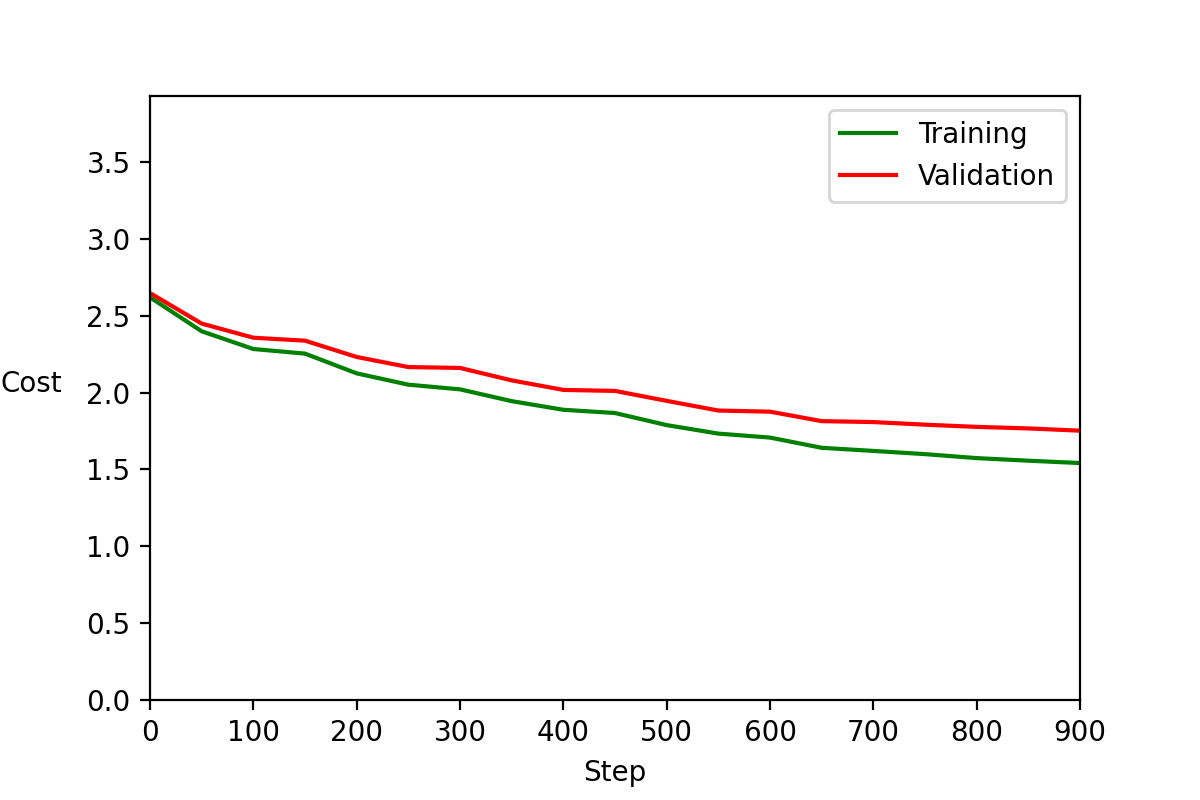
\includegraphics[width=4cm]{../plots/cost_init_v1.png}
		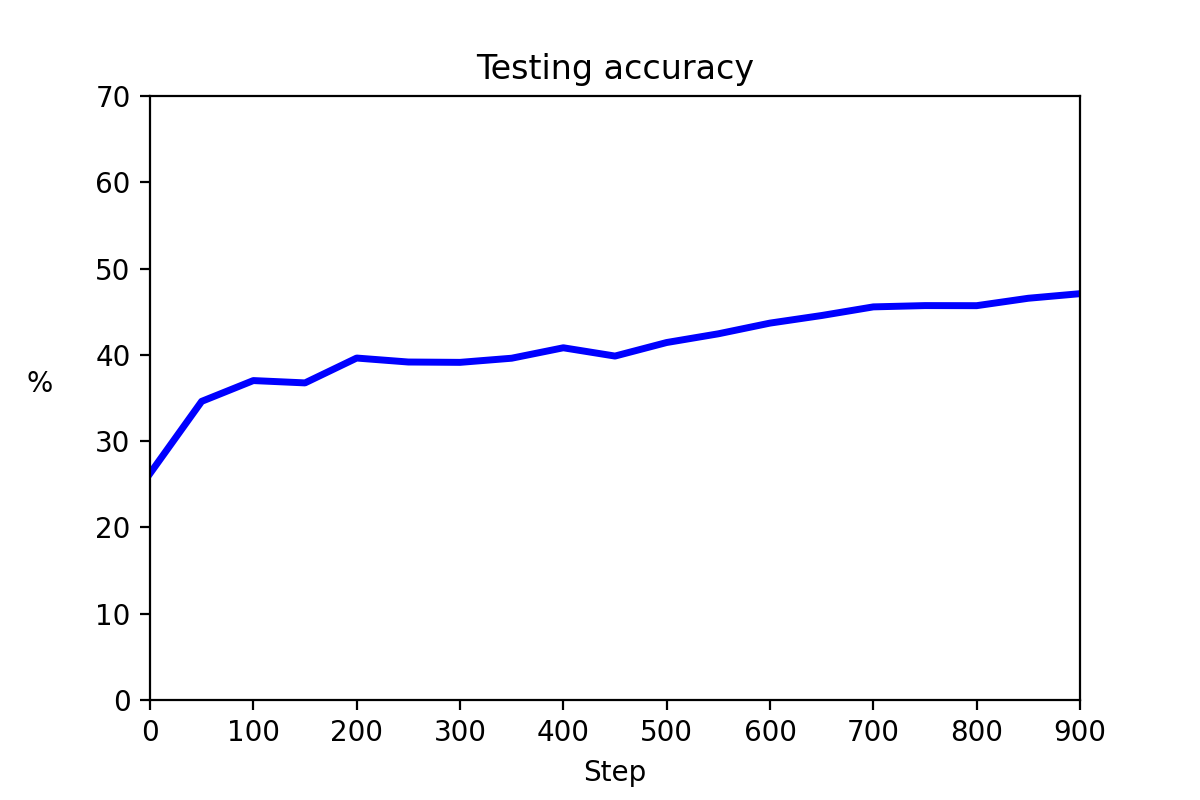
\includegraphics[width=4cm]{../plots/acc_init_v1.png}
		\caption{Loss, cost and accuracy for \texttt{etaMin}$=10^{-5}$, \texttt{etaMax}$=10^{-1}$, \texttt{nt}$=500$, and $1$ cycle.}
	\end{figure}		
	\begin{figure}[h!]
	%\vspace{0.1cm}
		\centering
		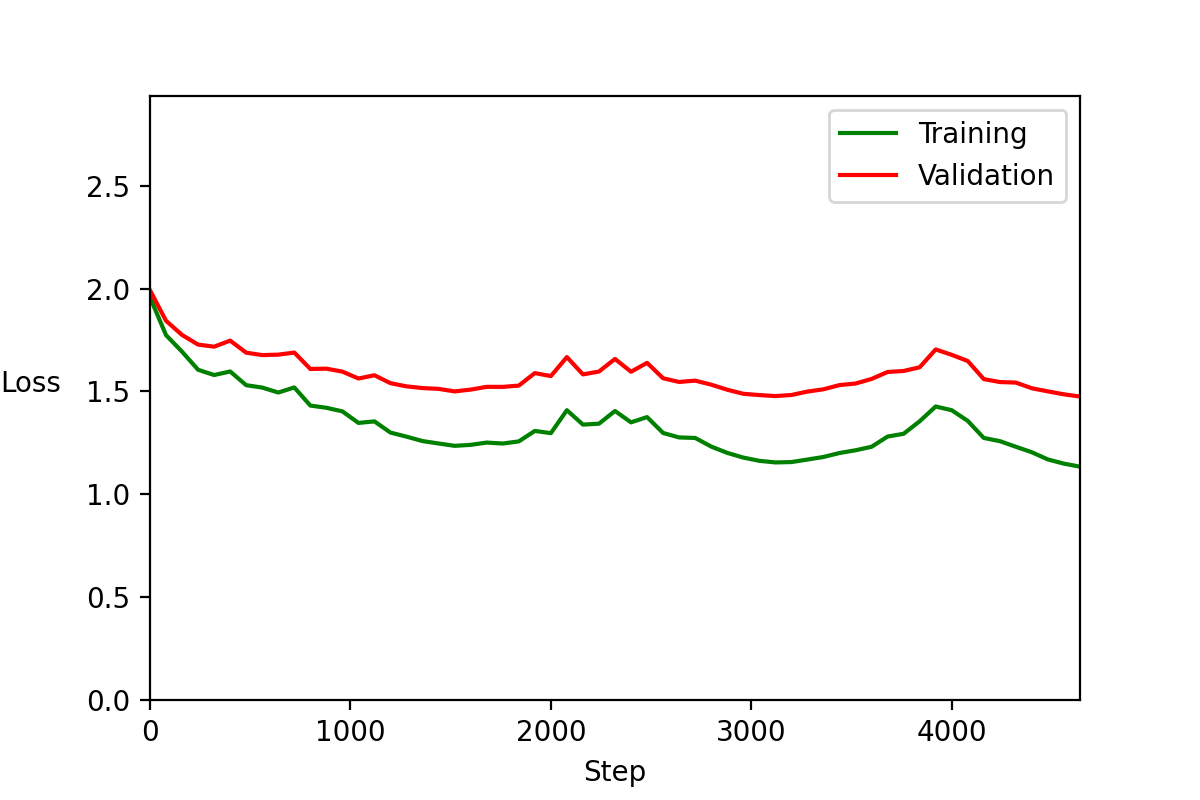
\includegraphics[width=4cm]{../plots/loss_init_v2.png}
		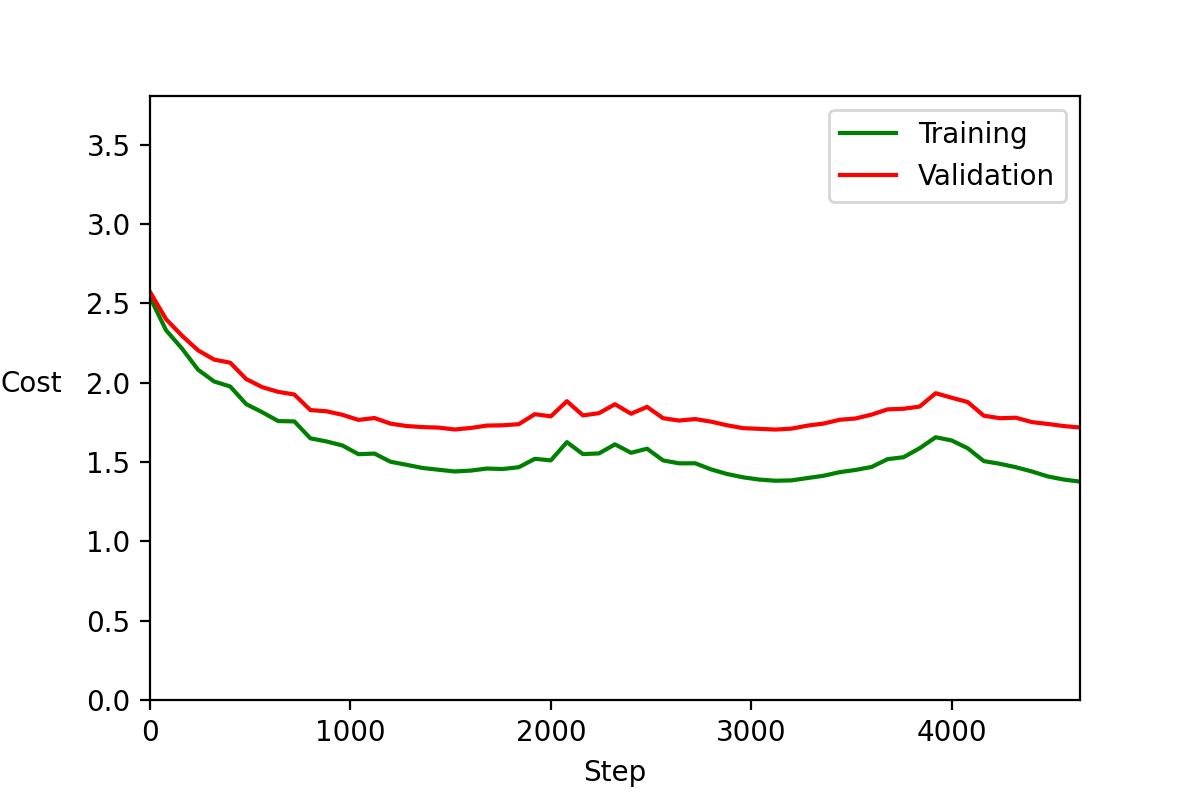
\includegraphics[width=4cm]{../plots/cost_init_v2.png}
		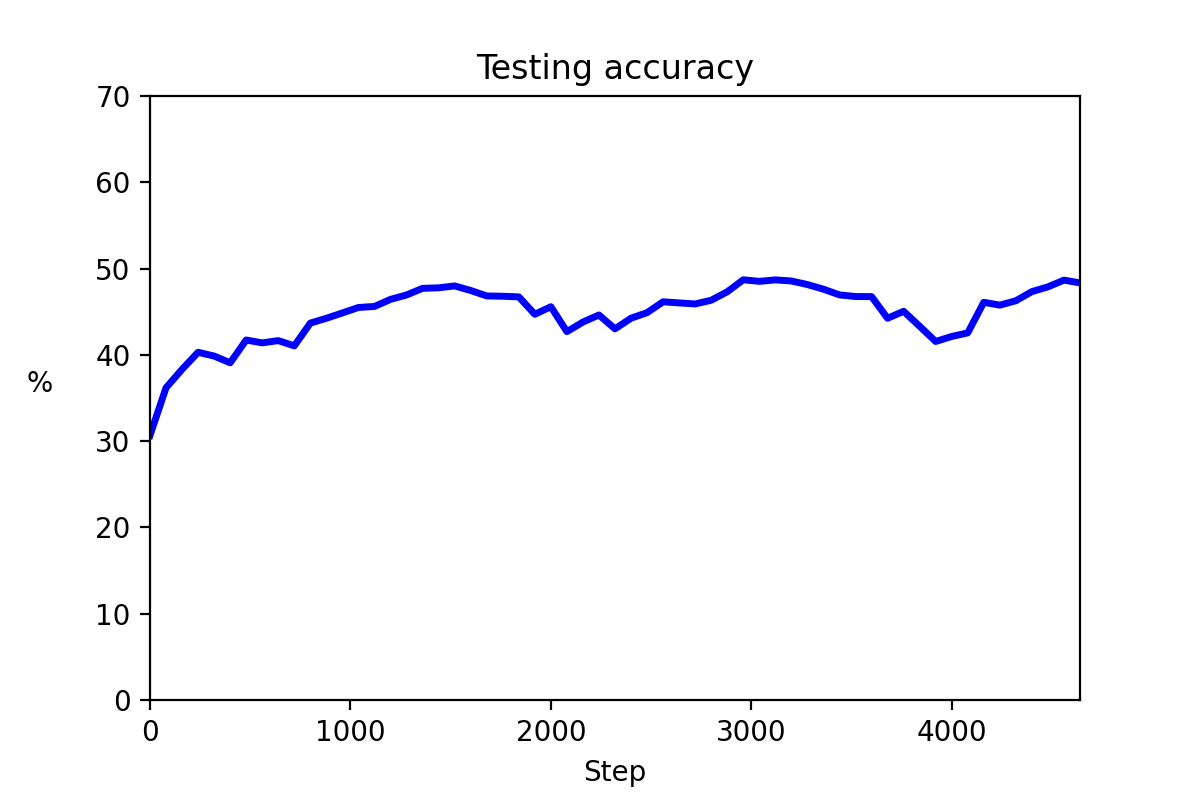
\includegraphics[width=4cm]{../plots/acc_init_v2.png}
		\caption{Loss, cost and accuracy for \texttt{etaMin}$=10^{-5}$, \texttt{etaMax}$=10^{-1}$, \texttt{nt}$=800$, and $3$ cycles.}
	\end{figure}\\

\subsection*{Searching for $\lambda$}
	When searching for an optimal value for the regularization parameter, $\lambda$, I computed $\texttt{nt}$ based on the size of the training data, which was $\vert D\vert = 45000$, and \texttt{nBatch}$=100$, such that \texttt{nt}$=450$. I then trained for $2$ cycles for each value of $\lambda$, which was calculated using
	$$\lambda = 10^{l}, \quad l = \lambda_{\text{min}} + (\lambda_{\text{max}} - \lambda_{\text{min}}) \cdot \bm{u}, \quad \bm{u}\sim\text{Uniform}(0, 1)$$
	where $\lambda_{\text{min}} = -5$ and $\lambda_{\text{max}} = -1$. The search was implemented with an initial coarse search, where $20$ different values of $\lambda$ were sampled. Then, the results from the coarse search were used to conduct a finer search. For the coarse search, the network seems to have performed worse with a higher $\lambda$, i.e. $\lambda > 0.01$. I have summarized the top-performing $\lambda$ settings in the following table. The same seed was used for all iterations.
	\begin{center}	
	\begin{tabular}{|l|c|}
		\hline
		 $\lambda$ & \text{Accuracy}, \% \\ \hline
		0.0005 & 51.16\\ 
		0.0003 & 51.15\\
		0.0026 & 51.14\\\hline
	\end{tabular}
	\end{center}
	Hence, for the fine search I instead set $\lambda_{\text{min}} = -5$ and $\lambda_{\text{max}} = -3$. The result for the three top-performing networks are shown in the table below. The performance gains are somewhat modest, with the best accuracy found in the fine search beats the one from the coarse search with only $+0.15$\%.  Finally, I trained a network for $5$ cycles, with \texttt{nt}$=500$ and $\lambda=0.0263$, for which the final accuracy on the test data was $51.80$\%. The results are plotted below in Figure $4$.
	
	\begin{center}	
	\begin{tabular}{|l|c|}
		\hline
		 $\lambda$ & \text{Accuracy}, \% \\ \hline
		0.00263 & 51.31\\ 
		0.0009 & 51.23\\
		0.002 	& 51.18\\\hline
	\end{tabular}
	\end{center}
	\begin{figure}[!h]
	%\vspace{0.1cm}
		\centering
		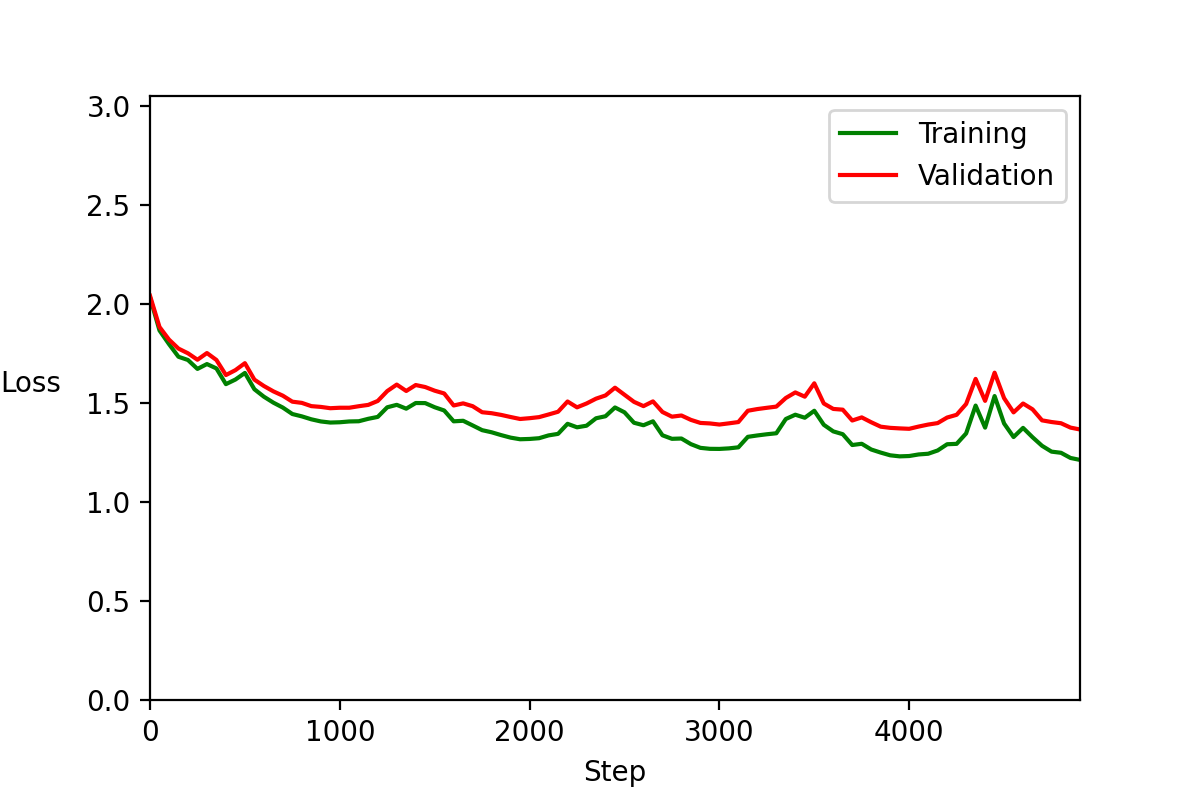
\includegraphics[width=4cm]{../plots/loss_top_v1.png}
		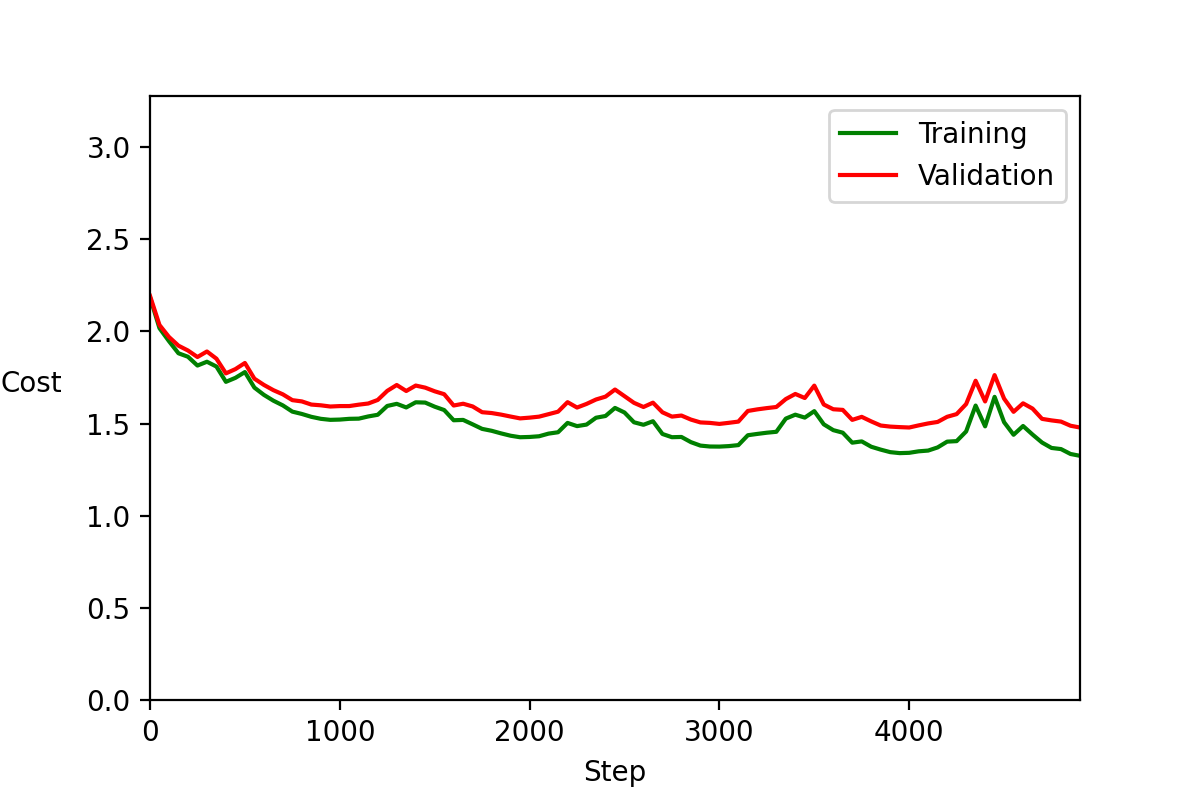
\includegraphics[width=4cm]{../plots/cost_top_v1.png}
		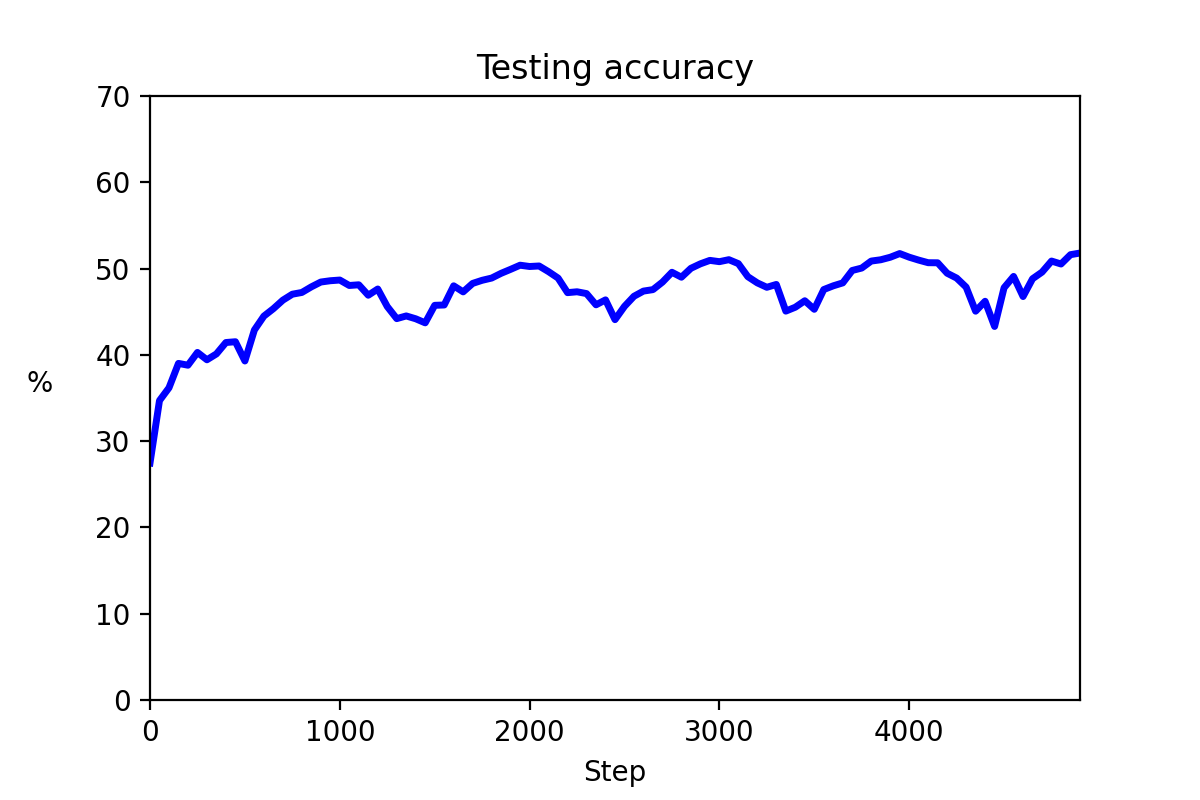
\includegraphics[width=4cm]{../plots/acc_top_v1.png}
		\caption{Loss, cost and accuracy for $\lambda=0.0263$, \texttt{etaMin}$=10^{-5}$, \texttt{etaMax}$=10^{-1}$, \texttt{nt}$=500$, and $5$ cycles.}
	\end{figure}


\end{document}